\documentclass[conference]{IEEEtran}
\IEEEoverridecommandlockouts
% The preceding line is only needed to identify funding in the first footnote. If that is unneeded, please comment it out.
\usepackage{cite}
\usepackage{amsmath,amssymb,amsfonts}
\usepackage{algorithmic}
\usepackage{graphicx}
\usepackage{textcomp}
\usepackage{tabularx}
\usepackage[table,xcdraw]{xcolor}

\begin{document}

\title{IoT based prediction of water quality index for farm irrigation}

\author{\IEEEauthorblockN{Rajesh Kumar Yadav}
\IEEEauthorblockA{\textit{Department of Computer Science and Engineering} \\
\textit{Delhi Technological University}\\
New Delhi-110042, India \\
rkyadav@dtu.ac.in}
\and
\IEEEauthorblockN{Adarsh Jha}
\IEEEauthorblockA{\textit{Department of Computer Science and Engineering} \\
\textit{Delhi Technological University}\\
New Delhi-110042, India \\
adarshjhaa100@gmail.com}
\and
\IEEEauthorblockN{\hspace{1.5cm}Aditya Choudhary}
\IEEEauthorblockA{\textit{\hspace{1.5cm}Department of Computer Science and Engineering} \\
\textit{\hspace{1.5cm}Delhi Technological University}\\
\hspace{1.5cm}New Delhi-110042, India \\
\hspace{1.5cm}adi20gamer@gmail.com}

}

\maketitle

\begin{abstract}
Agriculture sector of Indian economy in which more than half of the population is involved, contributes to less than quarter of the GDP. With advancement in ICT, tools and techniques can be developed that can help in analyzing and automating various phases of farming for improving productivity. This work focuses on analysing the quality of irrigation water and developing a model for prediction of Irrigation Water Quality Index(IWQI) based on Salinity and Sodicity.
Development of IWQI can save time and cost of lab tests for irrigation water. Five parameters of water Na$^+$, Cl$^-$, EC, HCO$^{3-}$ and SAR are measured using which the IWQI is calculated. These five parameters are further reduced to three parameters using correlation analysis and a classification model for prediction of water quality class is developed using various classification techniques. Best result is obtained by Random Forest Classifier followed by Gradient Boosting and Neural Network Classifier. The classification model can be used in IoT based farming systems for preventing salinity based damage to the crops.

\end{abstract}

\begin{IEEEkeywords}
Irrigation Water Quality Index, Precision Agriculture, Water salinity, Sensor Data
\end{IEEEkeywords}

\section{Introduction}
In a survey conducted in 2018, it was found that 50\% of the workforce in India is involved in the agriculture sector, however its contribution is only 16\% to the GDP\cite{article:indianEconomicSurvey}.There exists a need to increase the efficiency of each stage in farming and at a cheap cost so that it is affordable. With improvement in technology, these needs can be addressed using innovative solutions like the Internet of Things(IoT). This technology allows us to use sensors which in turn can be used to obtain large datasets for physical and chemical characteristics of soil, water and weather. This data can be analysed and machine learning tools can be developed that can help in proper utilization of resources and increase the overall efficiency of crop production. 

We require proper water quality standards for irrigation to improve crop yield and help maintain the soil productivity. Deficiency or excess of nutrients in soil also depends on water used for irrigation which effects the plant growth. However, most existing methods for water quality standards are for drinking water quality which is not suitable for plants and some methods which do exist for irrigation water quality use high number of parameters which ist't economically feasible for a farmer.


In this paper, we develop a model for prediction of Irrigation Water Quality Index(IWQI) class  based on the degree of sodicity and salinity of water. The contribution of our work are as follows:

\begin{itemize}
    \item We convert 5 parameters to quality measurement values which are used to calculate IWQI. We construct IWQI classes using IWQI values for irrigation water.
    \item  We reduce 5 parameters to 3 parameters using correlation analyis to save costs of sensors required to implement the proposed work. These parameters are used to classify IWQI using seven classification techniques which are Support Vector Classifier, Neural Networks, Gradient Boosting , Random Forest, Decision Tree, Bagging and Naive Bayes classifier.
    \item We evaluate and choose the best performing classification algorithm to obtain IWQI class for water sample with 3 parameters.
\end{itemize}

The rest of the paper is organized as follows: Section \ref{section:realtedWork} describes other works related to this paper, section \ref{section:preliminaries} discusses the preliminary topics, Section \ref{section:materialAndMethods} describes the database used and algorithm of the model, Section \ref{section:expAndRes} describes the results and finally Section \ref{section:conclusionAndFutureWork}  gives the conclusion and future work.

\section{Related Works}
\label{section:realtedWork}
With advancement in IoT, many new tools and techniques have been developed for agriculture sector. The term Precision agriculture\cite{article:precisionAgriculture} was developed in which various types of data such as time series, geolocation, sensor etc. are gathered and analysed to improve the efficiency of agricultural practices. Irrigation is one of the important phases of agriculture which involves adding water to soil after plantation which needs proper analysis of chemicals in water and quality of water for proper plant growth. 
 
Rajesh et al\cite{article:iotBasedIrrigationSystem} proposed an automated system that measures the moisture, temperature and humidity of farms measured using sensors to determine the optimal water volume required for Irrigation. Mark et al.\cite{article:water&soilwithconductivity} studied the effect of saline water on plants and proposed methods for using them for irrigation while Shrivastav et al.\cite{article:shrivastavSalinity} studied the effect of salinity on soil nutrients which decreases with increase in salinity due to its ability to reduce soil permeability. 

Irrigation Water quality Indices(IWQIs) are one way to aggregate various parameters of water samples into a single value and determine their suitability for irrigation. Meireles et al\cite{article:agricultureWQI} developed a WQI for irrigation water (which mainly focused on salinity and sodicity of water) using factor and principal component analysis to reduce thirteen parameters of water samples to just five parameters. Sayiter et al \cite{article:wqiModel1} used an Irrigation Water Quality Index(IWQI) using Sodium Adsorption Ratio (SAR), Kelly Index(KI), sodium percentage and Permeability Index(PI) and developed a model using Neural Networks for prediction of IWQI. Singh et al\cite{article:wqiModel2} uses index based approach for predicting water quality based on 12 parameters to classify water into 5 categories: excellent, good, medium, bad, and very bad. For performing this classification, they use multiple criteria decision analysis (MCDA) approach, indicating the importance of IWQI for managing water quality index. Hossam et al \cite{article:wqiModel3} used various dimensional reduction techniques such as Principal Component Analysis(PCA) and Factor Analysis(FA) to reduce 22 water quality parameters to 7 parameters:Sodium, Zinc, pH, Bicarbonate, Astantine, Boron and Nitrate and derived their weights using PCA. In the proposed work, we use the the IWQI developed by Meireles et al\cite{article:agricultureWQI} and develop a classification model to predict the IWQI class. 



\section{Preliminaries}
\label{section:preliminaries}

\subsection{Salinity Based Irrigation Water Quality}
\label{subsection:devIWQI}
Calculation of water quality for irrigation is necessary to study its effect on plant and soil health. Water Quality Index (WQI) is used for representing the overall quality of water. It is the aggregate of various chemical and physical parameters of water and is calculated by multiplying relative weights of parameters with parameter value. The parameters chosen should be able to be measured in all the water sources used for irrigation. In this work, we use the Irrigation Water Quality Index (IWQI) based on salinity and sodicity of water. The following subsections describe the water quality parameters, their weights and formula for calculating IWQI. 



\subsubsection{Parameters for IWQI}
\label{subsubsection:WaterQualityParameters}
The IWQI used in this work was formulated by Meireles et al who reduced 13 parameters of water using Factor Analysis(FA) and Principal Component Analysis(PCA) to 5 parameters which are: Sodium, Chloride and Bicarbonate ion concentration, Sodium Absorption Ratio (SAR) and Electrical Conductivity(EC) \cite{article:irrigationWaterQuality}. Electrical conductivity is generally measured by passing current through solutions and the value of SAR is given by the combination of Calcium, Magnesium and Sodium ion concentration whose formula is given by Equation \ref{equation:sar}. It is the primary indicator of sodicity of water which affects the permeability of soil and water infiltration rate\cite{book:waterQualityAgri}. Both cases of water infiltration rate being too high or too low affects the growth of plants. The weights of the 5 parameters, which represents their contribution to water quality are converted to relative weights and are mentioned in Table \ref{table:wqiParams}.

\begin{equation}
\label{equation:sar}
    SAR = \frac{Na^+}{\sqrt{\frac{Ca^{2+} + Mg^{2+}}{2}}} 
\end{equation}
Here, \newline
$Na^+$: Concentration of Sodium ion \newline
$Ca^{2+}$: Concentration of Calcium ion \newline
$Mg^{2+}$: Concentration of Magnesium ion \newline

\begin{table}[h!]
    \centering
    \caption{Weights for IWQI parameters}
    \begin{tabular}{|l|l|}
    \hline
        \textbf{Parameters} & \textbf{Weights} \\ \hline
        Electrical Conductivity(EC) & 0.211 \\ \hline
        Sodium(Na$^+$) & 0.204 \\ \hline
        Bicarbonate(HCO$^{3-}$) & 0.202 \\ \hline
        Chloride(Cl$^-$) & 0.194 \\ \hline
        Sodium Absorption Ratio (SAR) & 0.189 \\ \hline
    \end{tabular}
    \label{table:wqiParams}
\end{table}

\subsubsection{Quality Measurement Values and IWQI}
\label{subsubsection:calcIWQI}
The value of parameters measured for water sample should neither be too high nor too low for optimal growth of plants due to which the parameters are normalized(between 0 to 100) to quality measurement values ($q_i$) according to limits shown in Table \ref{table:qvalues}\cite{article:irrigationWaterQuality} and Equation \ref{equation:calcQ}. The $q_i$ values obtained are multiplied with relative weights of their respective parameters and finally added to obtain IWQI according to Equation \ref{equation:calcWQI} whose value is between 0 and 100. IWQI range is divided into various classes and each class represents the salinity characteristic. 




\begin{equation}
\label{equation:calcQ}
    q_i = q_{imax} - \frac{(x_{ij} - x_{inf})*q_{iamp}}{x_{amp}}
\end{equation} 
Here, \newline
$q_i$: quality measurement values, \newline
$q_{imax}$: maximum value in particular quality measurement class, \newline	
$q_{iamp}$: amplitude of quality measurement class, \newline
$x_{ij}$: value of parameter x, \newline
$x_{inf}$: minimum value of parameter x in quality measurement class, \newline
$x_{amp}$: It is the class amplitude to which the parameter belong 	

\begin{equation}
\label{equation:calcWQI}
    IWQI = \sum_{i=1}^{n}q_iw_i
\end{equation}
Here, \newline
$q_i$: quality measurement value , \newline
$w_i$: weight of parameter from Table \ref{table:wqiParams}

\begin{table}[h!]
    \centering
    \caption{Classification of water sample based on IWQI}
    \begin{tabular}{| m{0.1\linewidth} | m{0.35\linewidth} | m{0.35\linewidth} |}
    \hline
        \textbf{IWQI}  & \textbf{Soil} & \textbf{Plant} \\ \hline
        85–100 & Can be used for any kind of soil & Most plants won’t be affected \\ \hline
        70–85 & Can be used on soil with moderate permeability & Avoid use in plants with very low salt tolerance \\ \hline
        55–70 & Can be used on soils with moderate to high permeability & Avoid in plants with low salt tolerance \\ \hline
        40–55  & Can be used on soils with high permeability without dense layers & Used mainly in plants with high salt tolerance. Plants with moderate salt tolerance can be used with some control practices \\ \hline
        0–40 & Use for irrigation should be avoided & Avoid for all plants \\ \hline
    \end{tabular}
    \label{table:classifyWQI}
\end{table}

\begin{table}[h!]
    \centering
    \caption{Limiting values for quality measurement}
    \begin{tabular}{|m{0.075\linewidth}|m{0.13\linewidth}|m{0.13\linewidth}|m{0.12\linewidth}|m{0.12\linewidth}|m{0.13\linewidth}|}
    \hline
        \boldmath$q_{i}$ & \textbf{EC} & \textbf{SAR} & \boldmath{$Na^+$} & \boldmath{$Cl^-$} & \boldmath{$HCO^{3-}$} \\ \hline
        85-100 & 0.2\le{EC<0.75} & 2\le{SAR<3} & 2\le{$Na^+<3$} & 1\le{$Cl^-<4$} & 1\le{$HCO^{3-}<1.5$} \\ \hline
        60-85 & 0.75\le{EC<1.5} & 3\le{SAR<6} & 3\le{$Na^+<6$} & 4\le{$Cl^-<7$} & 1.5\le{$HCO^{3-}<4.5$} \\ \hline
        35-60 & 1.50\le{EC<3} & 6\le{SAR<12} & 6\le{$Na^+<9$} & 7\le{$Cl^-<10$} & 4.5\le{$HCO^{3-}<8.5$} \\ \hline
        0-35 & $EC<0.20$ or EC \ge 3.00 & $SAR<2$ or SAR\ge21 & $Na^+<2$ or $Na^+$\ge9 & $Cl^-<1$ or $Cl^-$\ge10 & $HCO^{3-}<1$ or $HCO^{3-}$\ge8.5 \\ \hline
    \end{tabular}
    \label{table:qvalues}
\end{table}

\subsection{Classification Algorithms}
\label{subsection:classificationAlgos}

\subsubsection{ANN}
\label{subsubsection:ann}
In ANN, we have an input layer, hidden layers and output layer each consisting of neurons in it\cite{book:ann}. Neurons receive some input and give an output after applying an activation function. The error is backpropagated to network for adjusting weights. This classifier is also known as MLP(Multilayer Perceptron Classifier).

\subsubsection{SVM}
\label{subsubsection:svm}
This classification algorithm is very useful as it tries to maximize the margin between any two classes which makes the decision hyperplane more accurate\cite{article:svm}. 

\subsubsection{Gradient Boost Classifier}
\label{subsubsection:gradientBoost}
It is a classifier which uses loss function, weak learners and an additive component to reduce the loss\cite{article:gradientBoosting}. This algorithm uses decision trees as its weak learners. It is quite powerful but is prone to overfitting.

\subsubsection{Random Forest Classifier}
\label{subsubsection:randomForestClassifier}
It is an ensemble learning method which uses multiple trees\cite{article:randomForest}. Here each classifier gives its own output and the output which is chosen by more number of classifiers becomes the final output.

\subsubsection{Decision Tree}
\label{subsubsection:decisionTree}
It is a classifier which uses a tree-like structure where at each node a decision is made according to the feature in the dataset and final output is given by the leaf node\cite{article:decisionTree}.


\subsubsection{Naive Bayes}
\label{subsubsection:naiveBayes}
It is a simple classifier which uses Bayes theorem with an exception that features do not depend on each other\cite{article:naiveBayes}. This allows us to easily implement and use the algorithm for classification but its results are not reliable.  

\subsubsection{Bagging Classifier}
\label{subsubsection:baggingClassifier}
This algorithm uses weak learners like decision trees on a random portion of its dataset, using the results from those trees to produce a final result\cite{article:baggingClassifier}. 


\section{Proposed Work}
\label{section:materialAndMethods}

\begin{figure}[h!]
\centering
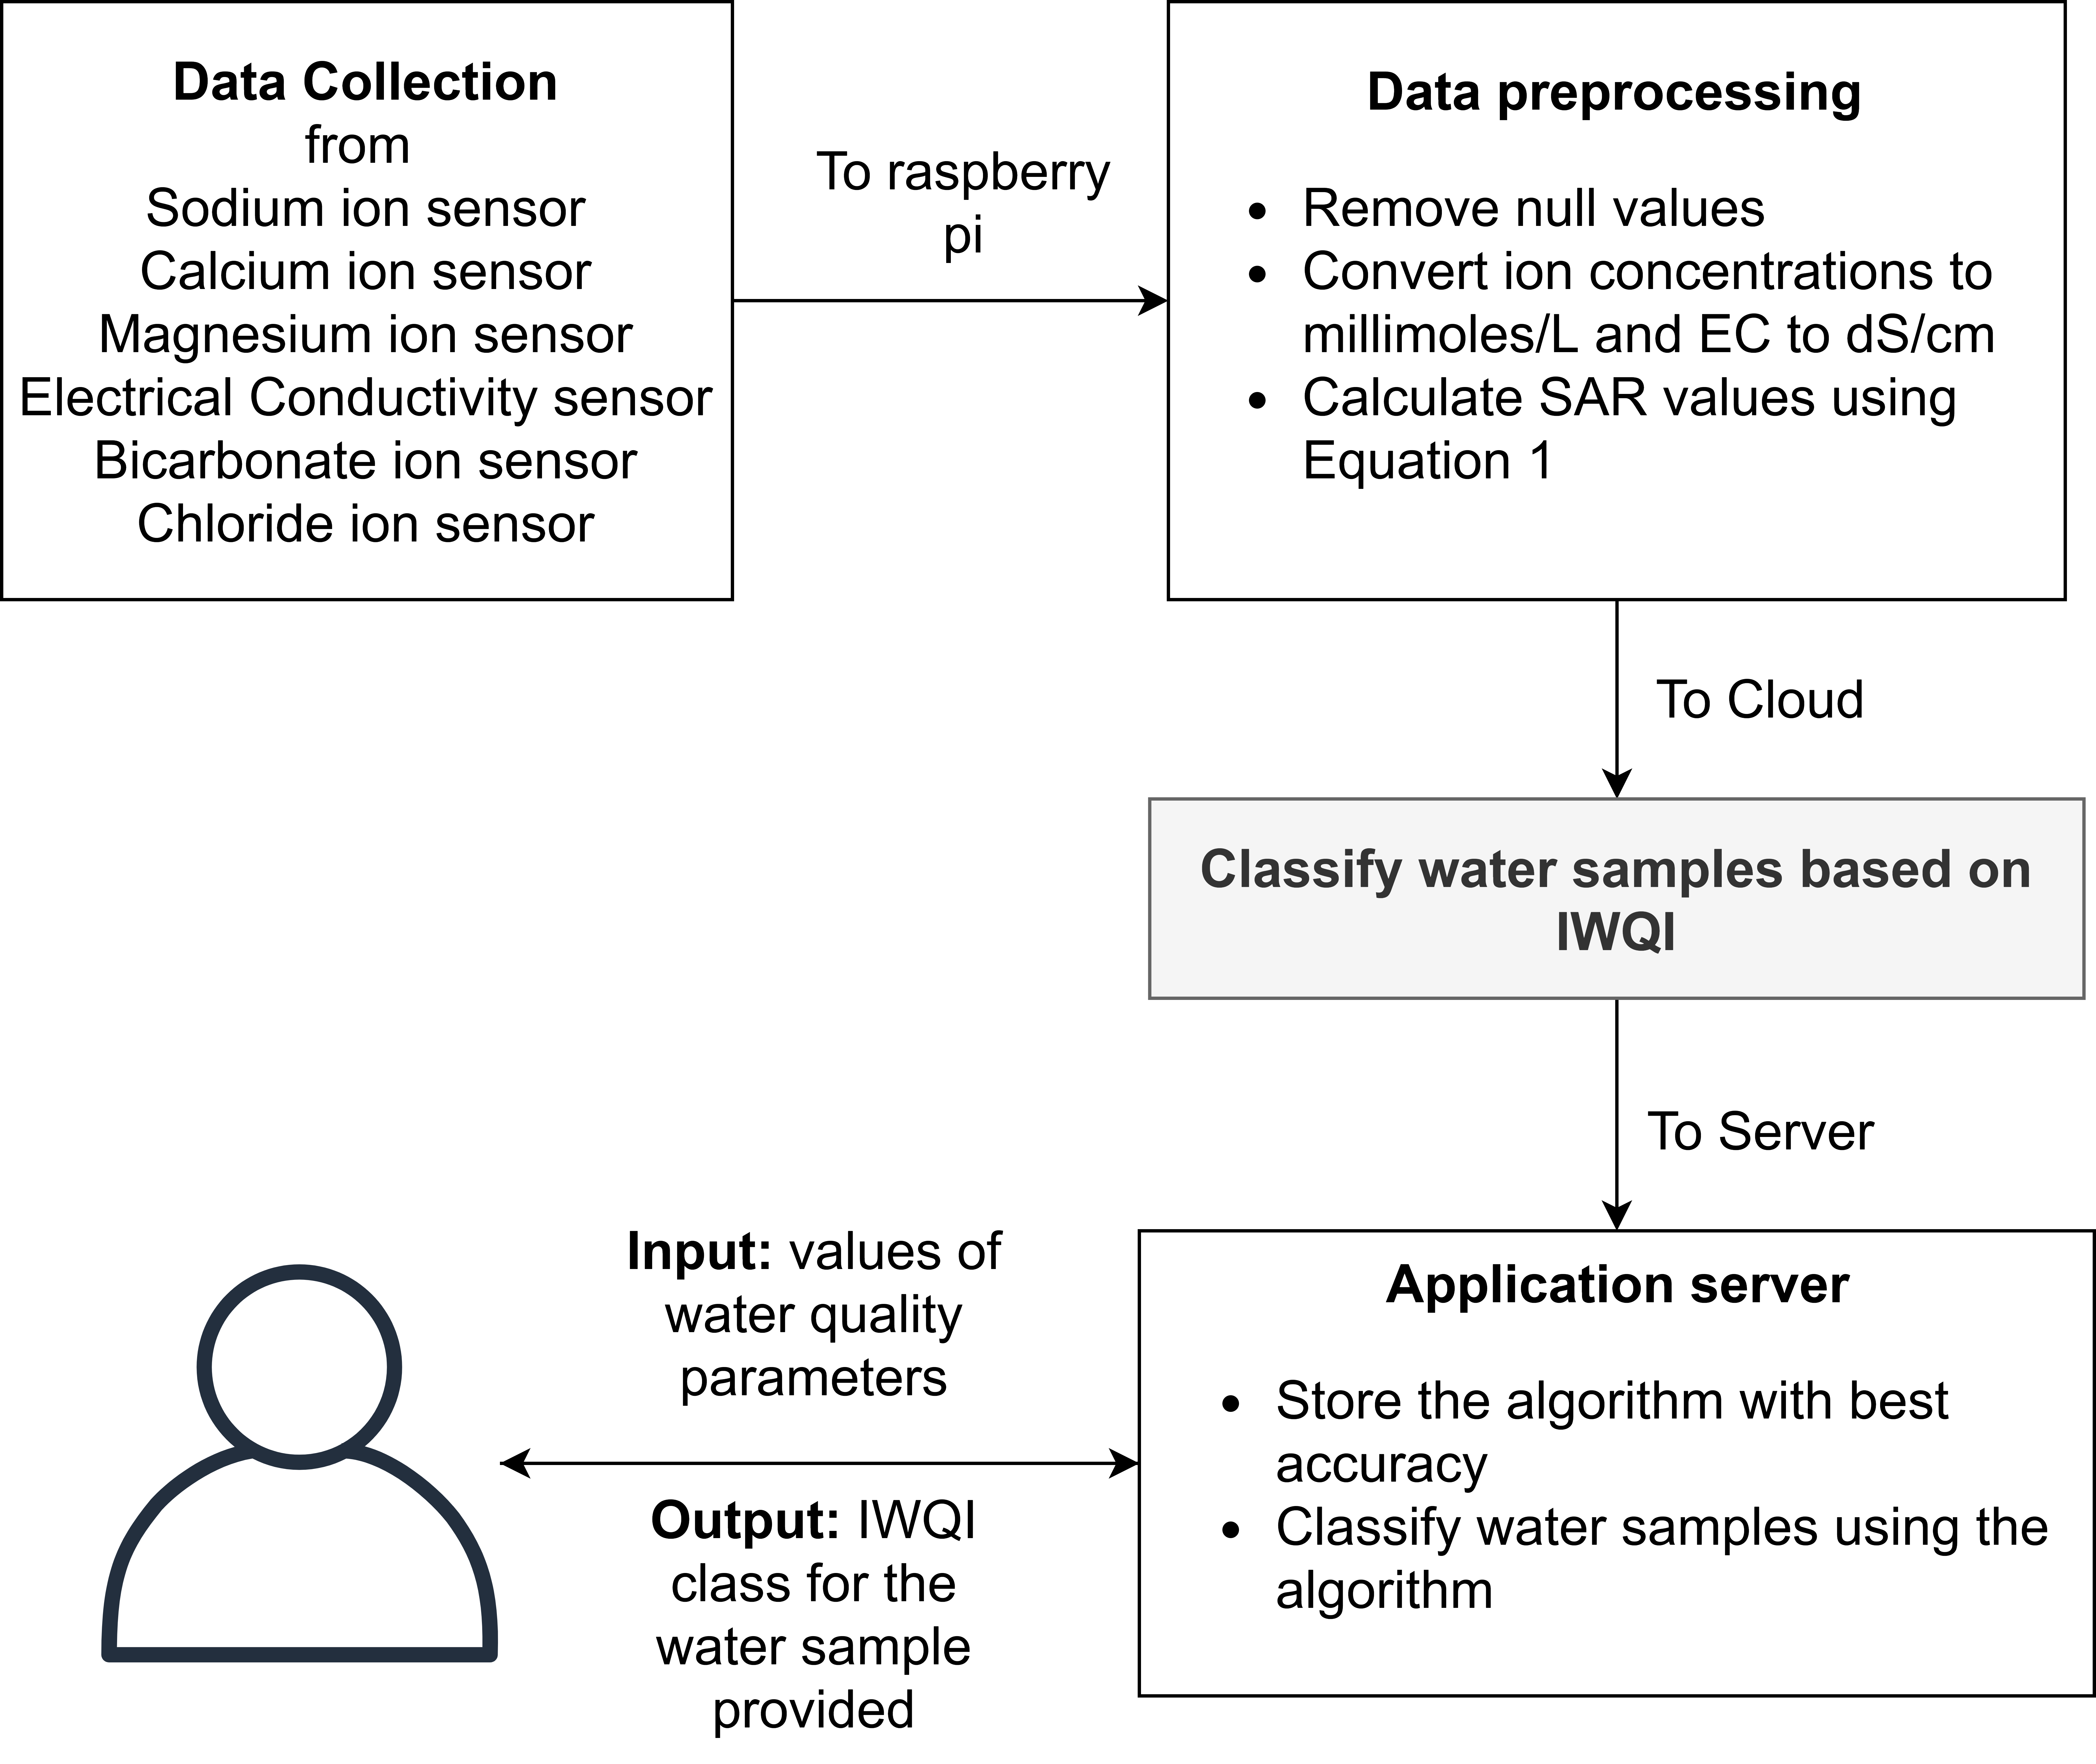
\includegraphics[width=8.5cm]{overallArchitecture.png}
\caption{Overall architecture}
\label{fig:overallArchitecture}
\end{figure}

In this section, we propose a classification model for prediction based on the Irrigation Water Quality(IWQI) class described in section \ref{subsubsection:calcIWQI}. The model can be incorporated into agricultural IoT systems for analysing water samples for irrigation purposes as shown in Fig. \ref{fig:overallArchitecture}. The sensor network will be used to measure the values of various water quality parameters namely electrical conductivity and ion concentrations for Sodium, Magnesium, Calcium, Bicarbonate and Chloride. Data from sensor network is sent to a local machine like Raspberry pi that involves processing the data and sending it to the cloud. The cloud analyses the data by predicting the relationship between water quality parameters and the IWQI classes. Result of classification can be saved to an application server than can interact with users through web or mobile applications. In this work, we have focused on the data analysis part which involves developing the classification model described in section \ref{subsection:iwqiClassification} used the water quality data from major ions dataset \cite{dataset:majorIons} that is described in section \ref{subsection:datasets}.    


\subsection{Dataset - Major ions dataset}
\label{subsection:datasets}
The dataset used in our work was obtained from US Geological Survey of Brackish Groundwater\cite{dataset:majorIons}. It consists of 66 thousand rows and contains values for concentration of dissolve solids, metals, nutrients, ions and physical properties such as conductivity out of which only EC, Cl$^-$, Na$^+$, HCO$^{3-}$, Ca$^{2+}$ and Mg$^{2+}$ are used for IWQI. EC stands for electrical conductivity which is measured in milliSiemens/cm. Cl$^-$, Na$^+$, HCO$^{3-}$, Ca$^{2+}$ and Mg$^{2+}$ represents  Chloride, Sodium, Bicarbonate, Calcium and Magnesium ion concentration respectively. These concentrations were measured in mg/L which we converted to millimoles/L. EC needs to be in dS/cm so it was divided by 100. We use Ca$^{2+}$, Mg$^{2+}$ and Na$^+$ to calculate SAR using Equation \ref{equation:sar}.


\subsection{Irrigation Water Quality Index based classification}
\label{subsection:iwqiClassification}
In this work, we develop a classification model and apply it on major ions dataset. This dataset consists of all the necessary features required to obtain the IWQI described in Section \ref{subsubsection:WaterQualityParameters} and the model is built using these three steps: converting given values to quality measurement values, calculating irrigation water quality index(IWQI) using calculated values and relative weights of each parameter, assigning to a class according to ranges given in Table \ref{table:classifyWQI} and finally using different classification techniques and choosing the best of them.

\subsubsection{Quality Measurement Values}
\label{subsubsection: QualityMeasurementValues}
The dataset consists of parameters with different units. Also, the value of any parameter being abnormally high or low decrease the quality of water. Hence, we need to normalize the values according to predefined limits of parameters. This is done by converting values of parameters to quality measurement values ($q_i$) that can be obtained using Equation 2 and Table 3. The quality measurement value ($q_i$) is a dimensionless quantity which can then be combined with other parameters without considering units. The Table \ref{table:numQualityMesurementInrange} indicates the number of values present in specific ranges of $q_i$ for the dataset used. Here, we can see that majority samples have $q_i$ values of EC in the range 85-100, bicarbonate in the range 35-85 and Cl$^-$, Na$^+$ and SAR in the range 0-35. This indicates that most of the samples have optimal value of EC and either excess or deficit value of Cl$^-$, Na$^+$ and SAR.



\begin{table}[h!]
    \centering
    \caption{Number of Quality measurement values in each range}
    \begin{tabular}{|l|l|l|l|l|l|}
    \hline
        \boldmath{$q_i$} & \textbf{Q\_HCO$^{3-}$} & \textbf{Q\_EC} & \textbf{Q\_Cl$^-$} & \textbf{Q\_Na$^+$} & \textbf{Q\_SAR} \\ \hline
        0-35 & 5540 & 6580 & 32700 & 31400 & 32600 \\ \hline
        35-60 & 9950 & 0 & 0 & 0 & 794 \\ \hline
        60-85 & 20000 & 3500 & 0 & 2780 & 1950 \\ \hline
        85-100 & 2470 & 27900 & 5280 & 3810 & 2680 \\ \hline
    \end{tabular}
    \label{table:numQualityMesurementInrange}
\end{table}

\subsubsection{Calculating IWQI and developing a classification model}
\label{subsubsection:classificationBasedOnIWQI}
Using the quality measurement values calculated in section \ref{subsubsection:calcIWQI}, we multiply them by their relative weights mentioned in Table \ref{table:wqiParams} and add them to obtain IWQI according to Equation \ref{equation:calcWQI}. The samples are further classified into quality classes according to quality ranges provided in Table \ref{table:classifyWQI}. Correlation matrix of quality parameters which was obtained using Pearson’s Correlation is given in Table \ref{table:correlationMatrixOfIons&IWQI}.The following observations are made: 

\begin{enumerate}
    \item Cl$^-$ is highly correlated with EC and Na$^+$.
    \item Na$^+$ is highly correlated with all the parameters.
    \item EC is highly correlated with all the parameters except SAR.
    \item HCO$^{3-}$ is highly correlated with EC.
    \item IWQI is highly correlated with Cl$^-$, Na$^+$ and EC.
\end{enumerate}



\begin{equation}
    r = \frac{\sum(U_i - \Bar{U})(V_i - \Bar{V})}{\sqrt{\sum(U_i - \Bar{U})^2(V_i - \Bar{V})^2}}
\label{equation:correlationMatrixOfIons&IWQI}
\end{equation}

Here, \newline
r: correlation coefficient \newline
U$_i$: value of U-variable in the sample \newline
$\Bar{U}$: mean value of U-variable \newline
V$_i$: value of V-variable in the sample \newline
$\Bar{V}$: mean value of V-variable


\begin{table}[h!]
    \centering
    \caption{correlation matrix for various parameters for water samples}
    \begin{tabular}{|l|l|l|l|l|l|l|}
    \hline
         & Cl$^-$ & Na$^+$ & EC & HCO$^{3-}$ & SAR & IWQI \\ \hline
        Cl$^-$ & 1 & 0.467 & 0.506 & 0.159 & 0.083 & 0.44 \\ \hline
        Na$^+$ & 0.467 & 1 & 0.482 & 0.297 & 0.56 & 0.607 \\ \hline
        EC & 0.506 & 0.482 & 1 & 0.835 & 0.018 & 0.423 \\ \hline
        HCO$^{3-}$ & 0.159 & 0.297 & 0.835 & 1 & 0.018 & 0.293 \\ \hline
        SAR & 0.083 & 0.56 & 0.018 & 0.018 & 1 & 0.302 \\ \hline
        IWQI & 0.44 & 0.607 & 0.423 & 0.293 & 0.302 & 1 \\ \hline
    \end{tabular}
    
    \label{table:correlationMatrixOfIons&IWQI}
\end{table}

We used different combination of parameters according to their correlation with IWQI value as features to the classification model in which Na$^+$, Cl$^-$ and EC were found to be most suitable for prediction IWQI class. The classification result obtained using the three parameters are almost similar to that obtained using all of the five parameters. Therefore, correlation analysis is sufficient and other feature reduction techniques are not required. Choosing three parameters saves us the cost of measuring HCO$^{3-}$ and SAR. The classification algorithms mentioned in Section \ref{subsection:classificationAlgos}  are used to predict quality classes and the method having best accuracy and F2 score is selected for further use. Multiple classification techniques have been used to cover different traditional, ensemble and deep learning based techniques whose performance can help in predicting the most suitable type of classification technique for the given dataset. The overall algorithm is mentioned in algorithm \ref{algorithm:classifyIWQI} and flowchart in Fig. \ref{fig:classificationFlowchart}.


\begin{algorithm}
	\caption{Classification of water samples based on IWQI}
	\begin{algorithmic}[1]
	    \label{algorithm:classifyIWQI}
		\renewcommand{\algorithmicrequire}{\textbf{Input:}}
		\renewcommand{\algorithmicensure}{\textbf{Output:}}
		\REQUIRE Water quality dataset with 5 parameters Cl$^-$, Na$^+$, EC, HCO$^{3-}$ and SAR
		
		\ENSURE  algorithm with best score       
        \STATE Calculate quality measurement values(q$_{param}$) for each parameter.
        \STATE Calculate IWQI using the Equation \ref{equation:calcWQI} and assign classes from Table \ref{table:classifyWQI}
        \STATE Choose features of dataset as: features \xleftarrow{} Cl$^-$,Na$^+$,EC 
        \STATE Choose labels of dataset as:IWQI
        \STATE Perform train test split on the dataset
        \STATE Apply the 7 classifiers mentioned in Section \text{\ref{subsection:classificationAlgos}} on the training set and evaluate on the testing set using accuracy and F1 score.
        \RETURN algorithm with best score
        % \EndProcedure
	\end{algorithmic} 
\end{algorithm}

\begin{figure}[h!]
\centering
\includegraphics[width=8cm]{IWQI_prediction.png}
\caption{Flowchart for classification of water sample based on IWQI}
\label{fig:classificationFlowchart}
\end{figure}

\section{Experiments and Results}
\label{section:expAndRes}
This section contains the simulation settings for implementing the classification model in \ref{subsection:toolsAndSimulationSettings}, the evaluation methods for the model  
\ref{subsection:evaluationMetrics} and the results of algorithms in section \ref{subsection:resultsOfClassificationBasedOnIWQI}.
%change some references
\subsection{Tools and Simulation Settings}
\label{subsection:toolsAndSimulationSettings}
The IoT system for classifying water samples based on IWQI values that is shown in Fig. \ref{fig:overallArchitecture} requires measurement of various water quality parameters mentioned in section \ref{subsubsection:WaterQualityParameters}. As we are focused on the classification part, we obtain the parameters from the Major ions dataset described in section \ref{subsection:datasets}. The algorithm was implemented in Python 3 where data preprocessing is performed using Pandas \cite{article:pandas} and Numpy \cite{article:numpy}. Various classification algorithms are applied using Scikit-learn. The parameter settings for these algorithms are mentioned in section \ref{subsection:parameterSettings}.    


\subsection{Parameter Settings}
\label{subsection:parameterSettings}
The parameter settings for all the classification models are given in Table \ref{table:parametersClassifiers} and the parameters are described below:

\subsubsection{Decision Tree}
\label{subsubsection:decisionTree}
criterion: function to evaluate split quality, splitter: method used to split at each node, min\_sample\_split: least amount of samples required to split a non-leaf node 

\subsubsection{Naive Bayes}
\label{subsubsection:naivebayes}
alpha: the additive smoothing parameter, class\_prior: estimated probability for new class prediction, class\_count: number of samples under each class 

\subsubsection{Gradient Boosting}
\label{subsubsection:gradientboosting}
loss: function to optimize, learning\_rate: for changing contribution of trees to the result, N\_estimators: levels of boosting 

\subsubsection{Random Forest}
\label{subsubsection:randomForest}
n\_estimators: Amount of tree before voting, criterion: function to evaluate split quality, base\_estimator: base classifier to create sub estimator

\subsubsection{Support vector classifier}
\label{subsubsection:supportvectorclassifier}
C: Regularization, decision\_shape: decision function’s shape, tol: stopping tolerance

\subsubsection{Bagging Classifier}
\label{subsubsection:baggingClassifier}
base\_estimator: base classifier used to fit on random subdomains, n\_estimator: count of the base\_estimator

\subsubsection{MLP Classifier}
\label{subsubsection:mlpClassifier}
hidden\_layer\_sizes: array representing sizes of hidden layers, activation: output function of hidden layer, learning\_rate: step size of gradient descent 

\begin{table}[h!]
    \centering
    \caption{Parameter Settings for Classifiers}
    \begin{tabular}{|m{0.20\linewidth}|m{0.45\linewidth}|}
    \hline
        \textbf{Classifier} & \textbf{Parameter Settings} \\ \hline
        Bagging Classifier & base\_estimator:SVC, n\_estimators:10 \\ \hline
        DecisionTree & criterion: gini, splitter: best, min\_samples\_split: 2 \\ \hline
        Naive Bayes & alpha: 1.0, class\_prior: None, class\_count: [ 7059. 15826.  5057.  2055.   402.] \\ \hline
        Gradient Boosting & loss: deviance, learning rate: 0.1, n\_estimators: 100 \\ \hline
        Random Forest & n\_estimators: 100, criterion: gini, base\_estimator\_: DecisionTreeClassifier \\ \hline
        SVM & C: 1.0, decision\_function\_shape: 'ovr', tol:0.001 \\ \hline
        MLP & hidden\_layer\_sizes:128, activation='relu', learning\_rate=0.001 \\ \hline
    \end{tabular}
    \label{table:parametersClassifiers}
\end{table}

\subsection{Evaluation Metrics For Classification Model}
\label{subsection:evaluationMetrics}
For testing our classifier, we use precision, accuracy, recall and F1 score. These metrics are calculated to test the reliability and robustness of classifiers used . These metrics are defined in Section \ref{subsubsection:accuracy}, \ref{subsubsection:precision}, \ref{subsubsection:recall} and  \ref{subsubsection:f1score}\cite{article:evaluationMetrics}. The equations for the same are given at \ref{equation:accuracy}, \ref{equation:precision}, \ref{equation:recall} and \ref{equation:f1Score}. 

\subsubsection{Accuracy}
\label{subsubsection:accuracy}
It tell us how much data can be predicted accurately from a given classifier. This gives us an idea about the bulk of data which is correctly classified.

\subsubsection{Precision}
\label{subsubsection:precision}
It tells us how many predictions are correct out of all observations saying output belongs to a particular class.

\subsubsection{Recall}
\label{subsubsection:recall}
It tells us how many correct predictions were made for a class out of all the actual observations for a given class.

\subsubsection{F1 Score}
\label{subsubsection:f1score}
It can be defined as harmonic mean of precision and recall, can be used independently for evaluation of classifiers.


\begin{equation}
\label{equation:accuracy}
    Accuracy = \frac{TPos + TNeg}{TPos + TNeg + FPos + FNeg}
\end{equation}

\begin{equation}
\label{equation:precision}
    Precision(P) = \frac{TPos}{TPos + FPos}
\end{equation}

\begin{equation}
\label{equation:recall}
    Recall(R) = \frac{TPos}{TPos + FNeg}
\end{equation}

\begin{equation}
\label{equation:f1Score}
    F1 Score = 2*\frac{P*R}{P+R}
\end{equation}
Here,\newline
TPos: Number of observations which are correctly classified for positive class in binary classification \newline
TNeg: Number of observations which are correctly classified for Negative class in binary classification \newline
FPos: Number of observations which are incorrectly classified for positive class in binary classification \newline
FNeg: Number of observations which are incorrectly classified for negative class in binary classification \newline

\subsection{Results of Classification based on IWQI}
\label{subsection:resultsOfClassificationBasedOnIWQI}
Algorithm \ref{algorithm:classifyIWQI} is applied to major ions dataset with Electrical Conductivity, Cl$^-$ and Na$^+$ as features and IWQI class as labels and results are evaluated using the metrics mentioned in Section \ref{subsection:evaluationMetrics}, details of which are mentioned in Section \ref{subsubsection:classificationBasedOnIWQI}. For the major ions dataset, the number of water samples in IWQI range 85-100 is around 1.3\% of the total samples which affected the results of correctly classifying samples belonging to that range. This however does not adversely affects the overall result. Random Forest performed the best with an accuracy of 86.9\% followed by Gradient Boosting and Neural Networks with accuracy of 85.8\% and 84.6\% respectively. Naive Bayes classifier performed the worst with accuracy of 52.6\%. The results of all the algorithms are given in Table \ref{table:classificationResults}. We also performed five-fold cross validation and computed the accuracies whose results are in Table \ref{table:fiveFoldCrossValidation}. This concludes that all of the methods except Naive Bayes perform well in classifying the water samples.
\begin{table}
    \centering
    \caption{Classification results for algorithm \ref{algorithm:classifyIWQI}}
    \begin{tabular}{|l|l|l|l|l|}
    \hline
        \textbf{Methods} & \textbf{Accuracy} & \textbf{Precision} & \textbf{Recall} & \textbf{F1} \\ \hline
        DecisionTree & 0.832 & 0.728 & 0.740 & 0.733 \\ \hline
        Naive Bayes & 0.526 & 0.105 & 0.200 & 0.138 \\ \hline
        Gradient Boosting & 0.858 & 0.762 & 0.757 & 0.760 \\ \hline
        Random Forest & \textbf{0.869} & \textbf{0.790} & \textbf{0.765} & \textbf{0.776} \\ \hline
        SVM & 0.845 & 0.762 & 0.711 & 0.726 \\ \hline
        Bagging & 0.813 & 0.750 & 0.664 & 0.690 \\ \hline
        MLP & 0.846 & 0.734 & 0.743 & 0.738 \\ \hline
    \end{tabular}
    \label{table:classificationResults}
\end{table}

\begin{table}
    \centering
    \caption{Five fold cross validation scores}
    \begin{tabular}{|m{0.25\linewidth}|m{0.09\linewidth}|m{0.09\linewidth}|m{0.09\linewidth}|m{0.09\linewidth}|m{0.09\linewidth}|}
    \hline
        \textbf{Methods} & \textbf{Fold 1} & \textbf{Fold 2} & \textbf{Fold 3} & \textbf{Fold 4} & \textbf{Fold 5} \\ \hline
        Bagging Classifier & 0.829 & 0.823 & 0.814 & 0.830 & 0.813 \\ \hline
        Decision Tree & 0.833 & 0.836 & 0.828 & 0.823 & 0.839 \\ \hline
        Naive Bayes & 0.518 & 0.518 & 0.518 & 0.518 & 0.519 \\ \hline
        Gradient Boosting & 0.862 & 0.866 & 0.869 & 0.859 & 0.862 \\ \hline
        Random Forest & \textbf{0.866} & \textbf{0.870} & \textbf{0.870} & \textbf{0.862} & \textbf{0.871} \\ \hline
        SVM & 0.853 & 0.849 & 0.846 & 0.841 & 0.848 \\ \hline
        MLP & 0.847 & 0.853 & 0.857 & 0.847 & 0.849 \\ \hline
    \end{tabular}
    \label{table:fiveFoldCrossValidation}
\end{table}



\section{Conclusion and Future Work}
\label{section:conclusionAndFutureWork}
Analysis of irrigation water quality can help in increasing agricultural productivity and prevent damage to plants. In this work, we developed a classification model for prediction of Irrigation Water Quality Index (IWQI) class. The IWQI used here is an aggregate of five parameters that are SAR, EC, Chloride, Bicarbonate and Sodium ion concentration respectively. For classification, we used seven classification algorithms and selected three out of five parameters: EC, Cl$^-$ and Na$^+$ for predicting IWQI class. Random Forest Classifier performed the best followed by Gradient Boosting and Neural Networks. The water quality index used here is mainly representation of salinity of water and the dataset used here is of groundwater. Other parameters such as acidity, oxygen demand etc. can be used in addition to the parameters used here to develop an index covering more factors. Also, dataset covering different types of water bodies can be used to improve the model. The proposed work used here can be incorporated into IoT based agricultural systems for analysing irrigation water quality that will be faster and economically feasible compared to manual lab tests. It can also help in deciding the water sample according to crop and soil properties.



\bibliographystyle{IEEEtran}      
\bibliography{references} 

\end{document}